\slides{STTI_intro_2017}{10}
\section{Muster vs Antimuster}
\lecdate{12.06.2017}
\subsection{Muster}
Wiederverwendung von \emph{Wissen} (Strukturen usw.)
\begin{itemize}
\item Entwurfs-Muster
\begin{itemize}
\item Erzeuger-Muster
\item Struktur-Muster
\item Verhaltens-Muster
\end{itemize}
\item Architektur-Muster
\begin{itemize}
\item 3-Säulen-Architektur
\item …
\end{itemize}
\end{itemize}
Typische Aufgabe $\to$ Lösungsvorschlag durch Muster
\subsection{Anti-Muster}
Ein Anti-Muster ist eine allgemein verbreitete Lösung einer Aufgabenstellung \emph{mit negativen Konsequenzen}.\\
Beschreibung von Anti-Mustern:
\begin{enumerate}
\item typische Aufgabenstellung
\item typische Lösungsvariablen mit negativen Konsequenzen
\item neu strukturieren:\\
$\to$ \emph{Refactoring}
\end{enumerate}
\subsection{Referenz-Modelle}
\begin{itemize}
\item Entwurfs-Muster
\begin{center}
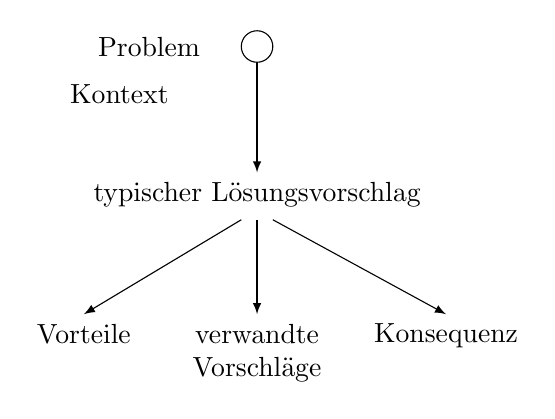
\begin{tikzpicture}[scale=.4]
\draw  (-2.5,4) ellipse (0.5 and 0.5);
\draw [-latex](-2.5,3.5) -- (-2.5,0) node[below]{typischer Lösungsvorschlag};
\node [left] at (-4,4) {Problem};
\node [left] at (-5,2.5) {Kontext};
\draw [-latex](-3,-1.5) -- (-8,-4.5) node[below]{Vorteile};
\draw [-latex](-2.5,-1.5) -- (-2.5,-4.5) node[below, align=center]{verwandte\\Vorschläge};
\draw [-latex](-2,-1.5) -- (3.5,-4.5) node[below]{Konsequenz};
\end{tikzpicture}
\end{center}
\item Anti-Muster\\
Lösung einer Aufgabenstellung mit Symptomen
\begin{center}
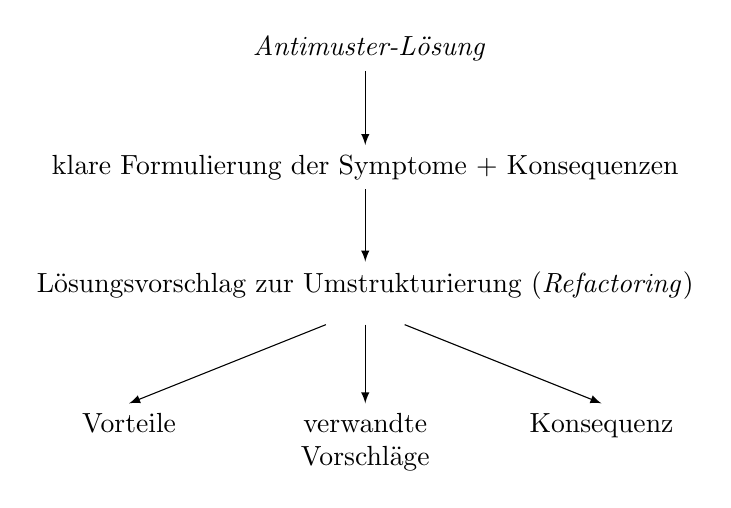
\begin{tikzpicture}
\node (v1) at (0,-1) {$\corr$ \emph{Antimuster-Lösung}};
\node (v2) at (0,-2.5) {klare Formulierung der Symptome + Konsequenzen};
\node (v3) at (0,-4) {Lösungsvorschlag zur Umstrukturierung (\emph{Refactoring})};
\draw [-latex](-0.5,-4.5) -- (-3,-5.5) node[below]{Vorteile};
\draw [-latex](0,-4.5) -- (0,-5.5) node[below, align=center]{verwandte\\Vorschläge};
\draw [-latex](0.5,-4.5) -- (3,-5.5) node[below]{Konsequenz};
\draw [-latex](v1) -- (v2);
\draw [-latex](v2) -- (v3);
\end{tikzpicture}
\end{center}
\end{itemize}

\section{Refactoring}
$\to$ Umstrukturierung\\
Möglichkeiten:
\begin{itemize}
\item Funktionalität (Verantwortlichkeit) in andere (neue) Klassen auslagern
\item neue Abstraktionsebenen einbauen: \\
$\to$ Superklasse extrahieren $\to$ Generalisierung (Vererbung)\\
$\to$ Subklassen bilden $\to$ Spezialisierung
\end{itemize}

\subsubsection*{Beispiel}
Von:
\begin{center}
\includegraphics[scale=.5]{Vorlesung/antipattern/Refactoring_davor.pdf}
\end{center}
Zu:
\begin{center}
\includegraphics[scale=.8]{Vorlesung/antipattern/Refactoring.pdf}
\end{center}

\section{Anti-Muster}

\subsection{The Blob}
\begin{itemize}
\item Symptom: riesengroße Klasse, die alles allein macht
\item Konsequenz: alle Änderungen beziehen sich auf diese Klasse
\item Ursache: nicht wirklich objektorientiert programmiert ($\to$ Objekte lösen gemeinsam eine Aufgabe)
\item Lösung: Attribute und zugehörige Funktionalitäten/Verantwortlichkeiten heraus finden und in neuer Klasse kapseln
\end{itemize}
falls Refactoring zu aufwändig:\\
$\to$ neuer Entwurf (Richtlinien: verteilte Verantwortlichkeit)\\
z.B.: CRC-Karten (Class Responsibility Collaboraters)\\
Im Kontrast dazu der „Anti-Blob“: Wenn zu viele Klassen existieren (jede Funktion eine Klasse)

\subsection{Lava Flow}
\begin{itemize}
\item Symptom: Quellcode der (wahrscheinlich) nicht mehr genutzt wird ($\to$ Dokumentation ???)
\item Ursache: 
\begin{itemize}
\item Lebensende Entwickler und keine wirkliche Übergabe.
\item prototypische Systeme werden als Produktiv-Systeme weiter entwickelt.
\item Vermischung von Laufzeit- und Persistenzobjekten.
\end{itemize}
\item Lösung: Ist-System dokumentieren $\to$ entsprechender Entwurf
\end{itemize}

\subsection{Poltergeister}
$\to$ Auftauchen und plötzliches Verschwinden
\begin{itemize}
\item Symptom: Klasse scheint wichtig, aber keiner weiß genau wofür
\item Ursache: 
\begin{itemize}
\item redundante Navigationspfade
\item „Helper-“, „Controller-“ Klassen
\item Zustandslose Klassen
\item …
\end{itemize}
\item Lösung: Poltergeister als Klasse beseitigen. Eventuell den Klassen zuordnen, von denen sie aufgerufen werden.
\end{itemize}

\lecdate{22.06.2017}

\subsection{Goldener Hammer}
$\to$ „Ich besitze einen Hammer („Wunderwaffe“) und alles andere sind Nägel.“

\begin{itemize}
\item Symptome:
\begin{itemize}
\item Die Architektur unseres Systems ist unsere Datenbank.
\item In der Analyse \emph{lenken} die Entwickler die Diskussion zu den Anforderungen aus der Perspektive der technologischen Lösungsmöglichkeiten.
\end{itemize}
\item Ursachen:
\begin{itemize}
\item aktuelle Entwicklung ist nicht im Blick
\item Überschätzung der bisherigen Lösungsvariante
\item blindes Vertrauen
\item hohe Investitionskosten müssen weiterhin die Technologiewahl bestimmen
\end{itemize}
\item Lösung:
\begin{itemize}
\item 2 Aspekte:
\begin{itemize}
\item Vorgehensweise (Kultur, philisophisch)\\
$\to$ Änderung im Entwicklungsprozess: Freiraum schaffen, Diskussion, Evaluieren
\item SW-System\\
Austauschbarkeit durch klare Abgrenzung der Komponenten (Abstraktionsstufe)
\end{itemize}
\end{itemize}
\end{itemize}


\subsection{Spaghetti-Code}
\begin{itemize}
\item Symptome:
\begin{itemize}
\item wenig Struktur im System
\item Objekt sind wie Prozess bezeichnet (mit Verb: bspw. \texttt{schreibt} anstatt \texttt{Schreiber})
\item Ablaufsteuerung ist vom Objekt, nicht vom Client des Objektes vorgeschrieben
\item Objektoperationen haben wenig bis keine Parameter (Instanziierung) $\to$ statt Parameter: 
\begin{itemize}
\item Klassenvariablen
\item globale Variablen
\end{itemize}
\end{itemize}
\item Ursachen:
\begin{itemize}
\item Sprachkonzepte sind nicht verstanden
\item vor Implementierungsphase gibt es keine Entwurfs-Phase
\item Entwickler arbeiten isoliert voneinander
\item keine Code-Überwachung
\end{itemize}
\item Lösung:
\begin{itemize}
\item Refactoring
\begin{itemize}
\item eher Prävention
\item ständige Code-Überwachung $\to$ wirkliches Refactoring: z.B. Objekte als Objekte verwenden
\end{itemize}
\end{itemize}
\end{itemize}

\section{Sotograph}
$=$ Plattform zur schnellen und komfortablen Untersuchung der inneren Struktur von SW-Systemen (für \lstinline`C / C++, Java, C#, ABAP, PHP, ...`)

\begin{center}
% TODO: Graphik aus prakt
\end{center}













